\subsection{Perkembangan empat eksperimen}
Tabel~\ref{tab:nb_tahap} membandingkan keempat eksperimen dengan Macro F1 OOF pada protokol tim. Kolom Public memuat skor leaderboard Kaggle untuk baseline 17 fitur, fine-tuning, dan varian kontekstual. Varian dua fitur yang mendahuluinya memakai \texttt{booking\_channel} dan \texttt{special\_requests} dan memperoleh 0,6652 OOF.

\begin{table}[H]
\centering
\caption{Hasil empat eksperimen Naive Bayes pada validasi dan Kaggle}
\label{tab:nb_tahap}
\begin{tabularx}{\textwidth}{p{3.0cm}Xrrrr}
\toprule
Tahap & Perubahan & Threshold & Macro F1 & Std fold & Public \\
\midrule
Baseline & 17 fitur asli, \(\alpha=1\) & 0,42 & 0,73422 & 0,00841 & 0,73697 \\
Fine-tuning & \(\alpha=2\), bobot fitur 2 & 0,49 & 0,73984 & 0,00482 & 0,74192 \\
Smoothing per\newline fitur & \(\alpha=10\) untuk permintaan & 0,49 & 0,73977 & 0,00460 & -- \\
Kontekstual & Bin kontekstual, 9 masukan & 0,43 & \textbf{0,80196} & 0,00729 & \textbf{0,80173} \\
\bottomrule
\end{tabularx}
\end{table}

\begin{figure}[htbp]
\centering
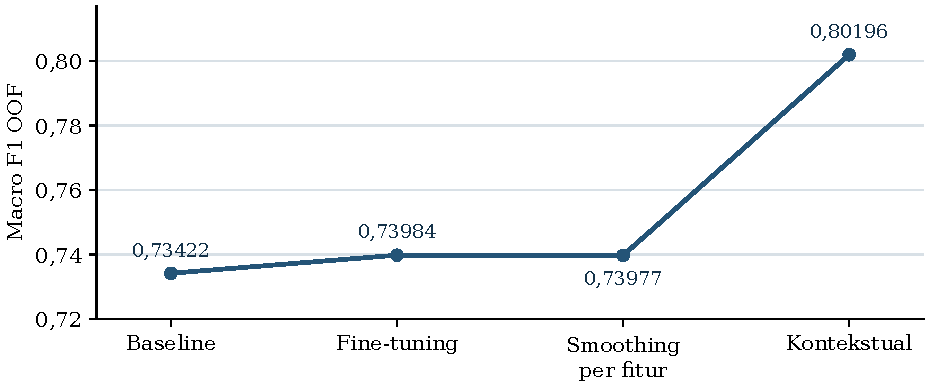
\includegraphics[width=0.84\textwidth]{nb_macro_f1.pdf}
\caption{Perubahan Macro F1 OOF antar-eksperimen pada protokol tim.}
\label{fig:nb_oof}
\end{figure}

Fine-tuning menaikkan Macro F1 sebesar 0,00562 dan memperbaiki empat dari lima fold. Dibanding baseline, false positive turun dari 3.917 ke 3.252, sedangkan false negative naik dari 2.688 ke 3.044. Smoothing per fitur menghasilkan perubahan total \(-0{,}00007\), walaupun tiga fold membaik tipis. Pada konfigurasi ini, smoothing yang lebih kuat untuk satu fitur belum menambah daya prediksi. Perubahan terbesar muncul pada tahap kontekstual, dengan kenaikan 0,06219 terhadap tahap sebelumnya. Karena tahap tersebut sekaligus mengubah diskretisasi, susunan fitur, dan pemilihan parameter, selisihnya mengukur efek gabungan.

\subsection{Validasi bertingkat dan perbandingan dengan scikit-learn}
Konfigurasi ekspor memperoleh OOF seleksi 0,80328 dengan threshold 0,45. Skor ini ikut menentukan konfigurasi yang dipilih. Validasi bertingkat memperoleh 0,79943 pada gabungan prediksi fold luar dan unggul pada lima fold terhadap \texttt{nb\_categorical\_tuned}, pembanding lama yang memakai bin hari rinci, kuantil tarif, dan gabungan kanal dengan rentang hari. Pembanding tersebut menggunakan prosedur validasi bertingkat yang sama dan berbeda dari baseline 17 fitur pada Tabel~\ref{tab:nb_tahap}.

\begin{table}[H]
\centering
\caption{Macro F1 pada fold luar validasi bertingkat kontekstual}
\label{tab:nb_nested}
\begin{tabular}{lrrr}
\toprule
Fold luar & Pembanding lama & Kontekstual & Threshold kontekstual \\
\midrule
1 & 0,75828 & 0,81082 & 0,435 \\
2 & 0,75328 & 0,79016 & 0,450 \\
3 & 0,75488 & 0,79297 & 0,475 \\
4 & 0,75433 & 0,80747 & 0,460 \\
5 & 0,74997 & 0,79571 & 0,420 \\
\midrule
OOF gabungan & 0,75421 & \textbf{0,79943} & -- \\
\bottomrule
\end{tabular}
\end{table}

\begin{table}[H]
\centering
\caption{Kesetaraan from scratch dengan pembanding scikit-learn pada konfigurasi yang sama}
\label{tab:nb}
\begin{tabularx}{\textwidth}{Xrrr}
\toprule
Tahap & From scratch & Pembanding & Selisih peluang maks. \\
\midrule
Baseline & 0,73422 & 0,73422 & \(6{,}00\times 10^{-15}\) \\
Fine-tuning (likelihood berbobot) & 0,73984 & 0,73984 & \(5{,}33\times 10^{-15}\) \\
Smoothing per fitur (likelihood berbobot) & 0,73977 & 0,73977 & \(5{,}44\times 10^{-15}\) \\
Kontekstual (OOF seleksi) & 0,80328 & 0,80328 & \(4{,}66\times 10^{-15}\) \\
\bottomrule
\end{tabularx}
\end{table}

Pada fine-tuning, \texttt{CategoricalNB} standar dengan bobot seragam dan \(\alpha=2\) memperoleh 0,73380. Pembanding berbobot memperoleh 0,73984. Selisih peluang pada Tabel~\ref{tab:nb} setara dengan galat pembulatan. Baris kontekstual memakai OOF seleksi karena verifikasi memakai konfigurasi ekspor dan fold yang sama.

\subsection{Analisis kesalahan, reproduksibilitas, dan bonus}
Prediksi gabungan fold luar kontekstual menghasilkan 15.960 \emph{true negative}, 2.444 \emph{false positive}, 2.400 \emph{false negative}, dan 6.569 \emph{true positive}. F1 kelas tidak batal mencapai 0,86824, sedangkan F1 kelas batal mencapai 0,73062. Pada kelompok \emph{lead time} lebih dari 80 hingga 151 hari, tingkat kesalahan masih 25,7\% dari 5.191 baris. Kelompok 11 hari atau kurang memiliki tingkat kesalahan 9,9\% dari 5.293 baris. Hasil ini menunjukkan bahwa kualitas prediksi berbeda antar-kelompok pemesanan setelah diskretisasi kontekstual.

Hasil run ulang \texttt{nb\_baseline} identik byte demi byte dengan \texttt{submission\_nb\_categorical\_all.csv} di branch \texttt{main}, yang mencatat public score 0,73697. Fine-tuning mencapai 0,74192 pada public leaderboard. Varian kontekstual mencapai 0,80173 dengan 6.844 prediksi dan threshold ekspor 0,45. Skor kontekstual 0,80196 dan 0,79943 berasal dari validasi data latih. KNN dengan vote booking kembar tetap menjadi model submission final kelompok.

Gambar~\ref{fig:nb_graf} menampilkan struktur dari sel bonus notebook kontekstual dengan label ringkas. Simpul \texttt{is\_canceled} memiliki sembilan anak sesuai masukan model. Panah menjelaskan faktorisasi peluang kondisional. Masing-masing simpul dapat berupa satu fitur atau satu kategori gabungan.

\begin{figure}[H]
\centering
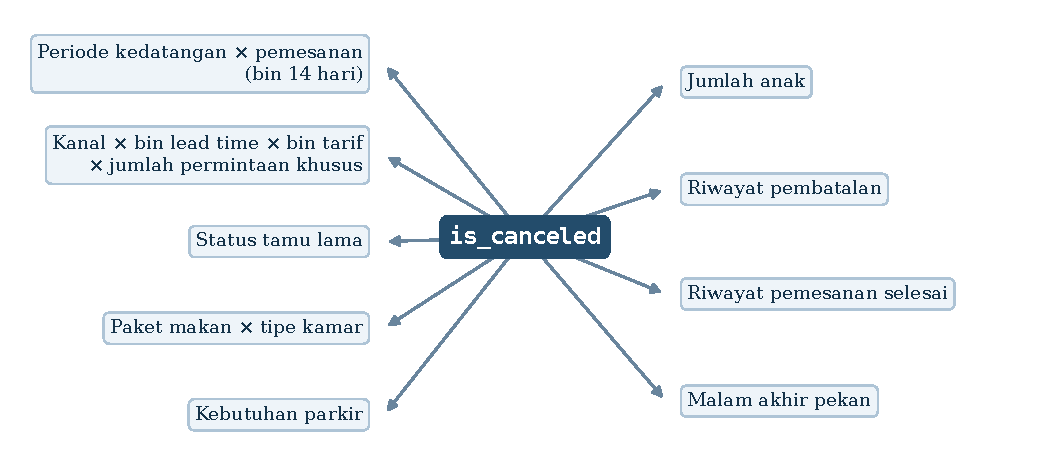
\includegraphics[width=\textwidth]{nb_graf.pdf}
\caption{Graf Bayesian Network untuk konfigurasi Categorical Naive Bayes kontekstual.}
\label{fig:nb_graf}
\end{figure}
